\documentclass{article}

\usepackage{amsmath}
\usepackage{amsfonts}
\usepackage{amssymb}
\usepackage{graphicx}
\usepackage[dvipsnames]{xcolor}
\usepackage[margin=0.5in]{geometry}
\usepackage[hidelinks]{hyperref}
\usepackage{enumitem}

\usepackage{array}

\graphicspath{{.}{./img/}}

\usepackage{environ}
\NewEnviron{centerframebox}{\begin{center}\fbox{\parbox{0.92\textwidth}{\BODY}}\end{center}}

\title{Algorithms for Data Science \\ Exercise Sheet 3}
\author{
  Vladislav Imashev \\ \href{mailto:s05vimas@uni-bonn.de}{s05vimas@uni-bonn.de} \and
  AAAAAAAAAA AAAAAAA \\ \href{mailto:AAAAAAAAAAAAAAAAAAAA}{AAAAAAAAAAAAAAAAAAAA} \and
  German Mikhelson \\ \href{mailto:s17gmikh@uni-bonn.de}{s17gmikh@uni-bonn.de} \and
  Aleksandra Volynets \\ \href{mailto:s02avoly@uni-bonn.de}{s02avoly@uni-bonn.de} \and
  Nikita Morev \\ \href{mailto:s99nmore@uni-bonn.de}{s99nmore@uni-bonn.de}
}

\begin{document}
  \maketitle

  \setcounter{section}{3}
  \subsection{Length of Frequent Itemsets}
  \begin{centerframebox}
    Prove the theorem on Slide 27 of 2023-11-08.
    \\\\
    \textbf{Theorem}:
    Given a transaction database $D$, an integer frequency threshold $t > 0$, and an integer $k > 0$,
    the problem of deciding if there is a frequent itemset consisting of at least $k$ items is NP-complete.
    \\\\
    \textit{Hint}: Consider the following problem and negative result:
    \textsc{Balanced Bipartite Clique Problem}:
    Given a bipartite graph $G = (V_1,\, V_2,\, E)$ and a positive integer $k$, decide whether $G$ has a balanced
    bipartite clique of size $k$, i.e., whether there are $V_1' \subseteq V_1$ and $V_2' \subseteq V_2$
    with $|V'_1| = |V'_2| = k$ such that $\{u,\, v\} \in E$ for all $u \in V'_1$ and for all $v \in V'_2$.
    \\\\
    Thm. (see Garey \& Johnson, 1979): The Balanced Bipartite Clique problem is NP-complete.
    \\\\
    You may prove the theorem by constructing a transactional database $\mathcal{D}$
    for a bipartite graph $G$ such that $G$ has a balanced bipartite clique of
    size $k$ if and only if $\mathcal{D}$ has a frequent itemset of cardinality $k$ for some
    appropriately chosen absolute frequency threshold $t$.
  \end{centerframebox}
  Let's reduce this problem to the \textsc{Balanced Bipartite Clique Problem}.

  Let's construct a transaction database $D$. We can represent the nodes in the bipartite graph as items in the transactional database. For every node in $V_1$ create a transaction consisting of this node and all the adjacent nodes in $V_2$. Let $t = k$.

  Example for $k = 2$:
  \begin{center}
    \begin{tabular}{ >{\centering\arraybackslash} m{0.4\textwidth}  >{\centering\arraybackslash} m{0.4\textwidth} }
      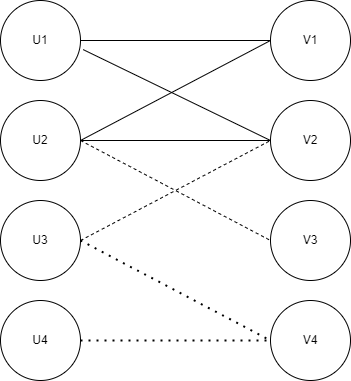
\includegraphics[width=0.3\textwidth]{task3.1_graph_drawio.png} &

      \begin{tabular}{|l|}\hline
        \textbf{Transaction Database $D$} \\\hline
        U1, \textbf{V1}, \textbf{V2} \\\hline
        U2, \textbf{V1}, \textbf{V2} \\\hline
        U3, V2, V4 \\\hline
        U4, V4 \\\hline
      \end{tabular}
    \end{tabular}
  \end{center}

  Now, we can show the equivalence between the existence of a balanced bipartite clique in $G$ and the presence of a frequent itemset in $D$:
  \begin{enumerate}
    \item If $G$ has a balanced bipartite clique of size $k$, then $D$ has a frequent itemset of cardinality $k$:

    If there exists a balanced bipartite clique of size $k$ in $G$, then every node in set $V_1'$ is connected to every node in set $V_2'$ within the clique.
    This means that the items corresponding to the nodes in $V_2'$ will form a frequent itemset of cardinality $k$ in $D$, because every item in $V_1'$ forms a transaction that includes every item in $V_2'$.
    Since the size of the clique is $k$ and $t = k$, there will be at least $t$ such transactions making this itemset of cardinality $k$ frequent.

    \item If $D$ has a frequent itemset of cardinality $k$, then $G$ has a balanced bipartite clique of size $k$:

    If there exists a frequent itemset of cardinality $k$ in $D$, then there are at least $t$ transactions in which the $k$ items appear together.
    These transactions correspond to edges in the bipartite graph $G$, and by considering the nodes corresponding to the items in the frequent itemset, we can construct a balanced bipartite clique of size $k$ in $G$.
  \end{enumerate}

  Therefore, by constructing the transactional database $D$ from the bipartite graph $G$ as described above, we can establish the equivalence between the existence of a balanced bipartite clique and the presence of a frequent itemset, reducing out problem to \textsc{Balanced Bipartite Clique Problem}.
  Since \textsc{Balanced Bipartite Clique Problem} is NP-complete (see Thm. Garey \& Johnson, 1979) Length of Frequent Itemsets problem is also NP-complete.

  \subsection{Borders of Theories and Frequent Itemset Mining}
  \begin{centerframebox}
    For a transaction database $\mathcal{D}$ over $I$ and frequency threshold $t > 0$, let $\mathcal{F}$
    denote the family of all frequent itemsets. Show that any (deterministic)
    algorithm computing $\mathcal{F}$ that has access to $\mathcal{D}$ only via the query
    \[\textit{``Is itemset X frequent?''}\]
    must evaluate this query for at least $|\operatorname{Bd}(\mathcal{F})|$ number of itemsets.
  \end{centerframebox}
  We will have to run the query for all items $X \in \operatorname{Bd}^-(\mathcal{F})$,
  because all of there subsets are frequent, and we can't use them to conclude that $X$ will be infrequent.
  The only way to get that information is to run the query on $X$.
  Even if we already know whether or not literally every other element in the tree is frequent or not.

  The same argument applies to the maximal frequent itemsets in $Y \in \operatorname{Bd}^+(\mathcal{F})$.
  Given the knowledge on the frequency status of every other possible itemset in the database,
  the two possibilities of \textit{``Y is frequent''} and \textit{``Y is infrequent''} are both possible and equally likely.
  It is actually impossible to tell apart\footnote{without running a query}
  an element of $\operatorname{Bd}^-(\mathcal{F})$ and $\operatorname{Bd}^+(\mathcal{F})$
  in this contrived best case scenario, because all the subsets of $X$ and $Y$ will be frequent and all the supersets infrequent.

  So we must run the query for all the elements in $\operatorname{Bd}^-(\mathcal{F})$ and $\operatorname{Bd}^+(\mathcal{F})$,
  i.e. at least $|\operatorname{Bd}(\mathcal{F})|$ times.

  \subsection{Borders of Theories and the Apriori Algorithm}
  \begin{centerframebox}
    Given $\mathcal{D}$ and $t$ as in Task 2, for how many itemsets $X$ is the query \textit{``Is itemset X frequent?''} evaluated by the Apriori algorithm?
  \end{centerframebox}
  The Apriori algorithm evaluates the frequency of each frequent itemset before outputting it, and it also evaluates some of the infrequent itemsets.
  So, at minimum, the number of queries is on the order of $O(|\mathcal{F}|)$ which is exponential of the size of the input database.

  Let's think about the infrequent itemsets that will be checked.
  For that, the itemset must appear in the candidates list and have all of it's subsets be frequent.
  But that will make it, by definition, an \textit{minimal} infrequent itemset and a member of $\operatorname{Bd}^-(\mathcal{F})$.
  So the Apriori algorithm will check exactly $|\mathcal{F}| + |\operatorname{Bd}^-(\mathcal{F})|$ itemsets for frequency.

  \subsection{Borders of Theories and Hypergraph Transversals}
  \begin{centerframebox}
    Prove the theorem on Slide 7 of 2023-11-15.

    \textbf{Theorem}: Let $S$ be a family of frequent itemsets. Then $\operatorname{Tr}(H(S)) = \operatorname{Bd}^{-}(cl(S))$.

    (hint: show first that $X \subseteq I$ is a transversal of $H(S) \iff X \not\in \operatorname{cl}(S)$)
  \end{centerframebox}
  % By definition, $Bd^{-}(cl(S))$ consists of infrequent items whose subitems are frequent and, at the same time, the infrequent items themselves do not belong to $cl(S)$, while by definition, $Bd^{+}(cl(S))$ consists only from frequent itemsets from which we can conclude that $cl(S)$ contains only frequent itemsets.

  The transversal set $H(S)$ is the set of elements not belonging to $Bd^{+}(cl(S))$, hence, its elements belong to the set $Bd^{-}(cl(S))$, hence, $H(S)$ consists of infrequent itemsets, hence, $Tr(H(S))$ will also be infrequent, since this is a set of minimal transversals that are infrequent. Remembering the definition of Minimal infrequent itemset, this is the set of minimal infrequent itemsets, namely negative border, i.e. $Bd^{-}(cl(S))$, hence, $Tr(H(S)) = Bd^{-}(cl(S))$.

  \subsection{The Dualize and Advance Algorithm }
  \begin{centerframebox}
    A database has the following five transactions:

    \begin{center}
      \begin{tabular}{|c|c|}
        \hline
        TID & items bought \\ \hline
        1 & M, O, N, K, E, Y \\ \hline
        2 & D, O, N, K, E, Y \\ \hline
        3 & M, A, K, E \\ \hline
        4 & M, U, C, K, Y \\ \hline
        5 & C, O, K, E \\ \hline
      \end{tabular}
    \end{center}

    \begin{enumerate}[label=(\roman*)]
      \item Generate all maximal frequent itemsets with the Dualize and Advance algorithm for minimum frequency threshold $t = 3$.
      Give $S_k$, $\overline{S_k}$, and $\operatorname{Tr}(\overline{S_k})$ for all iterations of the algorithm.
      \item Give all minimal infrequent itemsets (for $t = 3$).
    \end{enumerate}
  \end{centerframebox}

  (i) Let's set the following alphabet: $M < O < N < K < E < Y < D < A < U < S$.
  Before we get started, we should remove infrequently occurring elements from the alphabet, which are: $N, D, A, U, S$. So we will work with: $M < O < K < E < Y$. \\
  \\
  \textbf{Step 1:}
  In the first step, we put all the elements into $\overline{S_1}$ and put the same elements into $Tr(S_1)$.
  \begin{center}
    $S_1 = \emptyset$ \\
    $\overline{S_1} = \{MOKEY\}$ \\
    $Tr(S_1) = \{M,O,K,E,Y\}$
  \end{center}

  \textbf{Step 2:}
  At this point we take $M$, because it is the lowest element in our alphabet, and try to construct the most frequent set of elements that we will put into $S_2$. Our $\overline{S_2}$ is the inverted $S_2$.
  \begin{center}
    $S_2 = \{MK\}$ \\
    $\overline{S_2} = \{OEY\}$ \\
    $Tr(S_2) = \{O,E,Y\}$
  \end{center}

  \textbf{Step 3:}
  At this point we take $O$ and construct new the most frequent set of elements that we will put into $S_3$.
  \begin{center}
    $S_3 = \{MK, OKE\}$ \\
    $\overline{S_3} = \{OEY, MY\}$ \\
    $Tr(S_3) = \{Y, MO, ME\}$
  \end{center}

  \textbf{Step 4:}
  At this point we take $Y$, which is the only frequent transversal we have,
  and construct new the most frequent set of elements that we will put into $S_4$.
  \begin{center}
    $S_4 = \{MK, OKE, KY\}$ \\
    $\overline{S_4} = \{OEY, MY, MOE\}$ \\
    $Tr(S_4) = \{MY, MO, ME, YO, YE\}$
  \end{center}
  But all elements in $Tr(S_4)$ are infrequent, hence, $STOP$.
  \\
  \\
  \textbf{Answer:} (i): all maximal frequent itemsets is $\{MK, OKE, KY\}$ \\

  (ii) By
  \begin{center}
    \textbf{Theorem}: Let $S$ be a family of frequent itemsets. Then $\operatorname{Tr}(H(S)) = \operatorname{Bd}^{-}(cl(S))$.
  \end{center}
  We know that $\operatorname{Tr}(H(S))$ contains all minimal infrequent sets of elements and in our problem this $\operatorname{Tr}(H(S))$ is equal to $Tr(S_4)$. So the answer is: $\{MY, MO, ME, YO, YE\}$
\end{document}
